\documentclass[border=4pt]{standalone}
\usepackage{tikz}
\usetikzlibrary{positioning, arrows.meta, shapes.geometric, calc, fit, backgrounds}
\usepackage{amsmath,amssymb}
\begin{document}
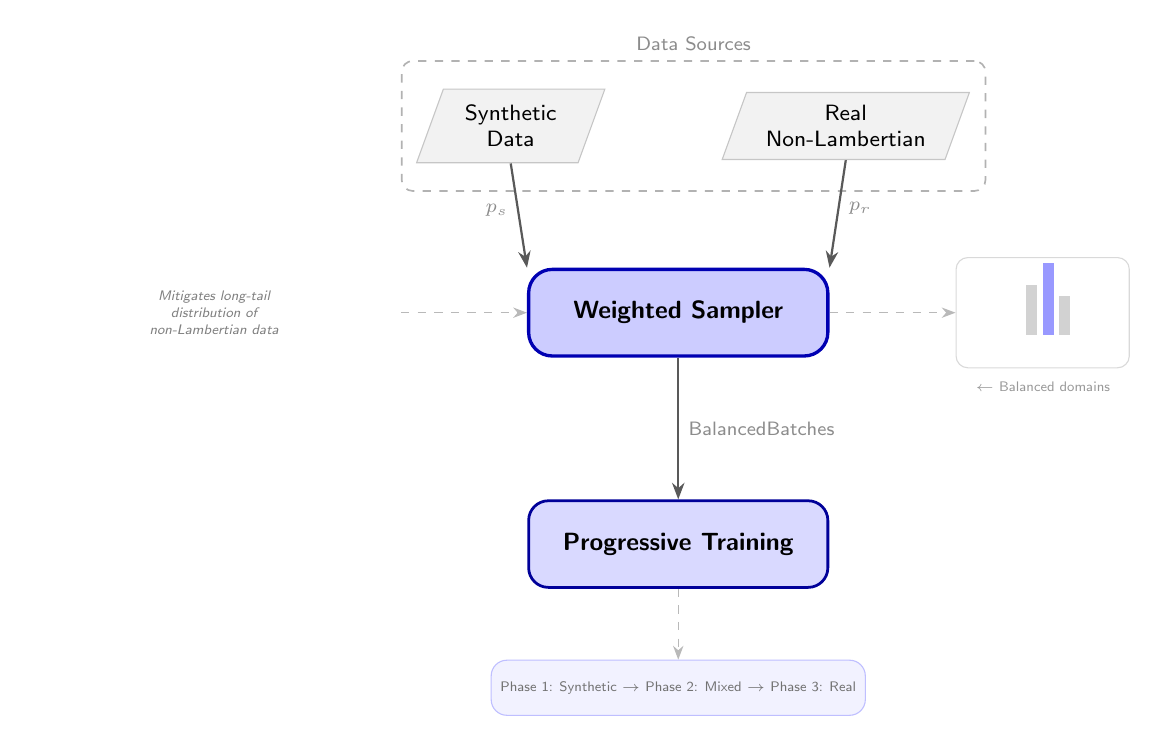
\begin{tikzpicture}[
  data/.style={draw, trapezium, trapezium left angle=70, trapezium right angle=110,
               minimum width=2.4cm, minimum height=0.85cm,
               fill=gray!10, draw=gray!45, align=center,
               font=\sffamily\footnotesize},
  innov/.style={draw, rounded corners=3mm, minimum width=3.8cm, minimum height=1.1cm,
                fill=blue!20, draw=blue!70!black, line width=1.2pt, align=center,
                font=\sffamily\small\bfseries},
  proc/.style={draw, rounded corners=2.5mm, minimum width=3.8cm, minimum height=1.1cm,
               fill=blue!15, draw=blue!60!black, line width=1pt, align=center,
               font=\sffamily\small\bfseries},
  arr/.style={-{Stealth[length=6pt]}, thick, color=black!65},
  arrd/.style={-{Stealth[length=5pt]}, dashed, color=gray!55},
  gbox/.style={draw=black!30, dashed, rounded corners=4pt, inner sep=10pt, line width=0.6pt},
  lbl/.style={font=\sffamily\scriptsize, text=black!45},
  annot/.style={font=\sffamily\tiny\itshape, text=black!50, align=center},
]

% === Data Sources (top row) ===
\node[data] (synth) {Synthetic\\Data};
\node[data, right=1.8cm of synth] (real) {Real\\Non-Lambertian};

% === Grouped box for data sources ===
\begin{scope}[on background layer]
  \node[gbox, fit=(synth)(real),
        label={[lbl]above:Data Sources}] (datasrc) {};
\end{scope}

% === Weighted Sampler (innovation) ===
\node[innov, below=1.8cm of $(synth)!0.5!(real)$] (sampler) {Weighted Sampler};

% === Progressive Training (innovation) ===
\node[proc, below=1.8cm of sampler] (training) {Progressive Training};

% === Annotation box for Progressive Training details ===
\node[draw=blue!25, rounded corners=2mm, fill=blue!5,
      minimum width=3.6cm, minimum height=0.7cm,
      align=center, font=\sffamily\tiny, text=black!55,
      below=0.9cm of training] (detail)
     {Phase~1: Synthetic $\rightarrow$ Phase~2: Mixed $\rightarrow$ Phase~3: Real};

% === Main arrows ===
\begin{scope}[on background layer]
  % Synth -> Sampler
  \draw[arr] (synth.south) -- node[lbl, left, pos=0.45] {$p_{s}$} (sampler.north west);
  % Real -> Sampler
  \draw[arr] (real.south) -- node[lbl, right, pos=0.45] {$p_{r}$} (sampler.north east);
  % Sampler -> Training
  \draw[arr] (sampler) -- node[lbl, right] {Balanced\\[-2pt]Batches} (training);
  % Training -> Detail
  \draw[arrd] (training) -- (detail);
\end{scope}

% === Annotation: long-tail note ===
\node[annot, text width=4.5cm,
      left=1.6cm of sampler, align=center]
     (annot1)
     {Mitigates long-tail\\distribution of\\non-Lambertian data};

% Dashed arrow from annotation to sampler
\begin{scope}[on background layer]
  \draw[arrd] (annot1.east) -- (sampler.west);
\end{scope}

% === Visual emphasis: small distribution diagram ===
% Mini bar chart annotation
\node[draw=gray!30, rounded corners=1.5mm, fill=white,
      minimum width=2.2cm, minimum height=1.4cm,
      right=1.6cm of sampler, align=center,
      inner sep=3pt] (distbox) {};

% Bars inside the distribution box using coordinates relative to distbox
\fill[gray!35] ([xshift=-6pt, yshift=-8pt]distbox.center) rectangle ([xshift=-2pt, yshift=10pt]distbox.center);
\fill[blue!40] ([xshift=0pt, yshift=-8pt]distbox.center) rectangle ([xshift=4pt, yshift=18pt]distbox.center);
\fill[gray!35] ([xshift=6pt, yshift=-8pt]distbox.center) rectangle ([xshift=10pt, yshift=6pt]distbox.center);

\node[font=\sffamily\tiny, text=black!40, below=0.05cm of distbox]
     {$\leftarrow$ Balanced domains};

\begin{scope}[on background layer]
  \draw[arrd] (sampler.east) -- (distbox.west);
\end{scope}

\end{tikzpicture}
\end{document}